\documentclass[11pt]{article}
\usepackage[margin=1in]{geometry}
\usepackage{graphicx}
\usepackage{booktabs}
\usepackage{float}
\usepackage{amsmath}
\usepackage{xcolor}
\usepackage[hidelinks]{hyperref}
\graphicspath{{figures/}}

\title{\textbf{Form S-6 Interactive Grid and Wind Fields}\\[2pt]
\large Sensitivity and Uncertainty Analysis over Southern Florida}
\author{Paul Fishwick and Claude Code}
\date{\today}

\begin{document}
\maketitle

\section{Purpose}
This project implements the grid and wind-field machinery underlying
\emph{Form S-6 (Hypothetical Events for Sensitivity and Uncertainty Analysis)} of
the Florida Commission on Hurricane Loss Projection Methodology Report of
Activities (ROA), which supports \emph{Standard S-3 (Uncertainty Analysis for
Hurricane Model Output)}. The deliverable is an interactive browser application
(HTML/CSS/JavaScript + Leaflet) that draws the official $21\times40$ grid over
southern Florida, runs selectable hurricane wind-field models over it, and
performs the sensitivity (SRC) and uncertainty (EPR) analyses the ROA prescribes.

\section{The grid and storm track}
The grid (ROA Figs.~3--4) has $21\times40=840$ vertices at $\sim$3 statute-mile
spacing: east--west $E\!=\!0,3,\dots,117$ (40 columns) and north--south
$N\!=\!-15,-12,\dots,45$ (21 rows). Of the 840 vertices, \textbf{682 are land}
and 158 water, taken directly from the \texttt{Land-Water ID} worksheet of
\texttt{FormS6Input.xlsx}. The point $(0,0)$ is the storm centre at $t\!=\!0$,
nine miles east of the landfall location $(25.8611^\circ$N$,\,80.1196^\circ$W$)$;
the storm tracks due west, $(0,0)\!\to\!(117,0)$, over 12 hours. Figure~\ref{fig:grid}
shows the rendered grid (land vs.\ water), the track, and the landfall marker.

\begin{figure}[H]
\centering
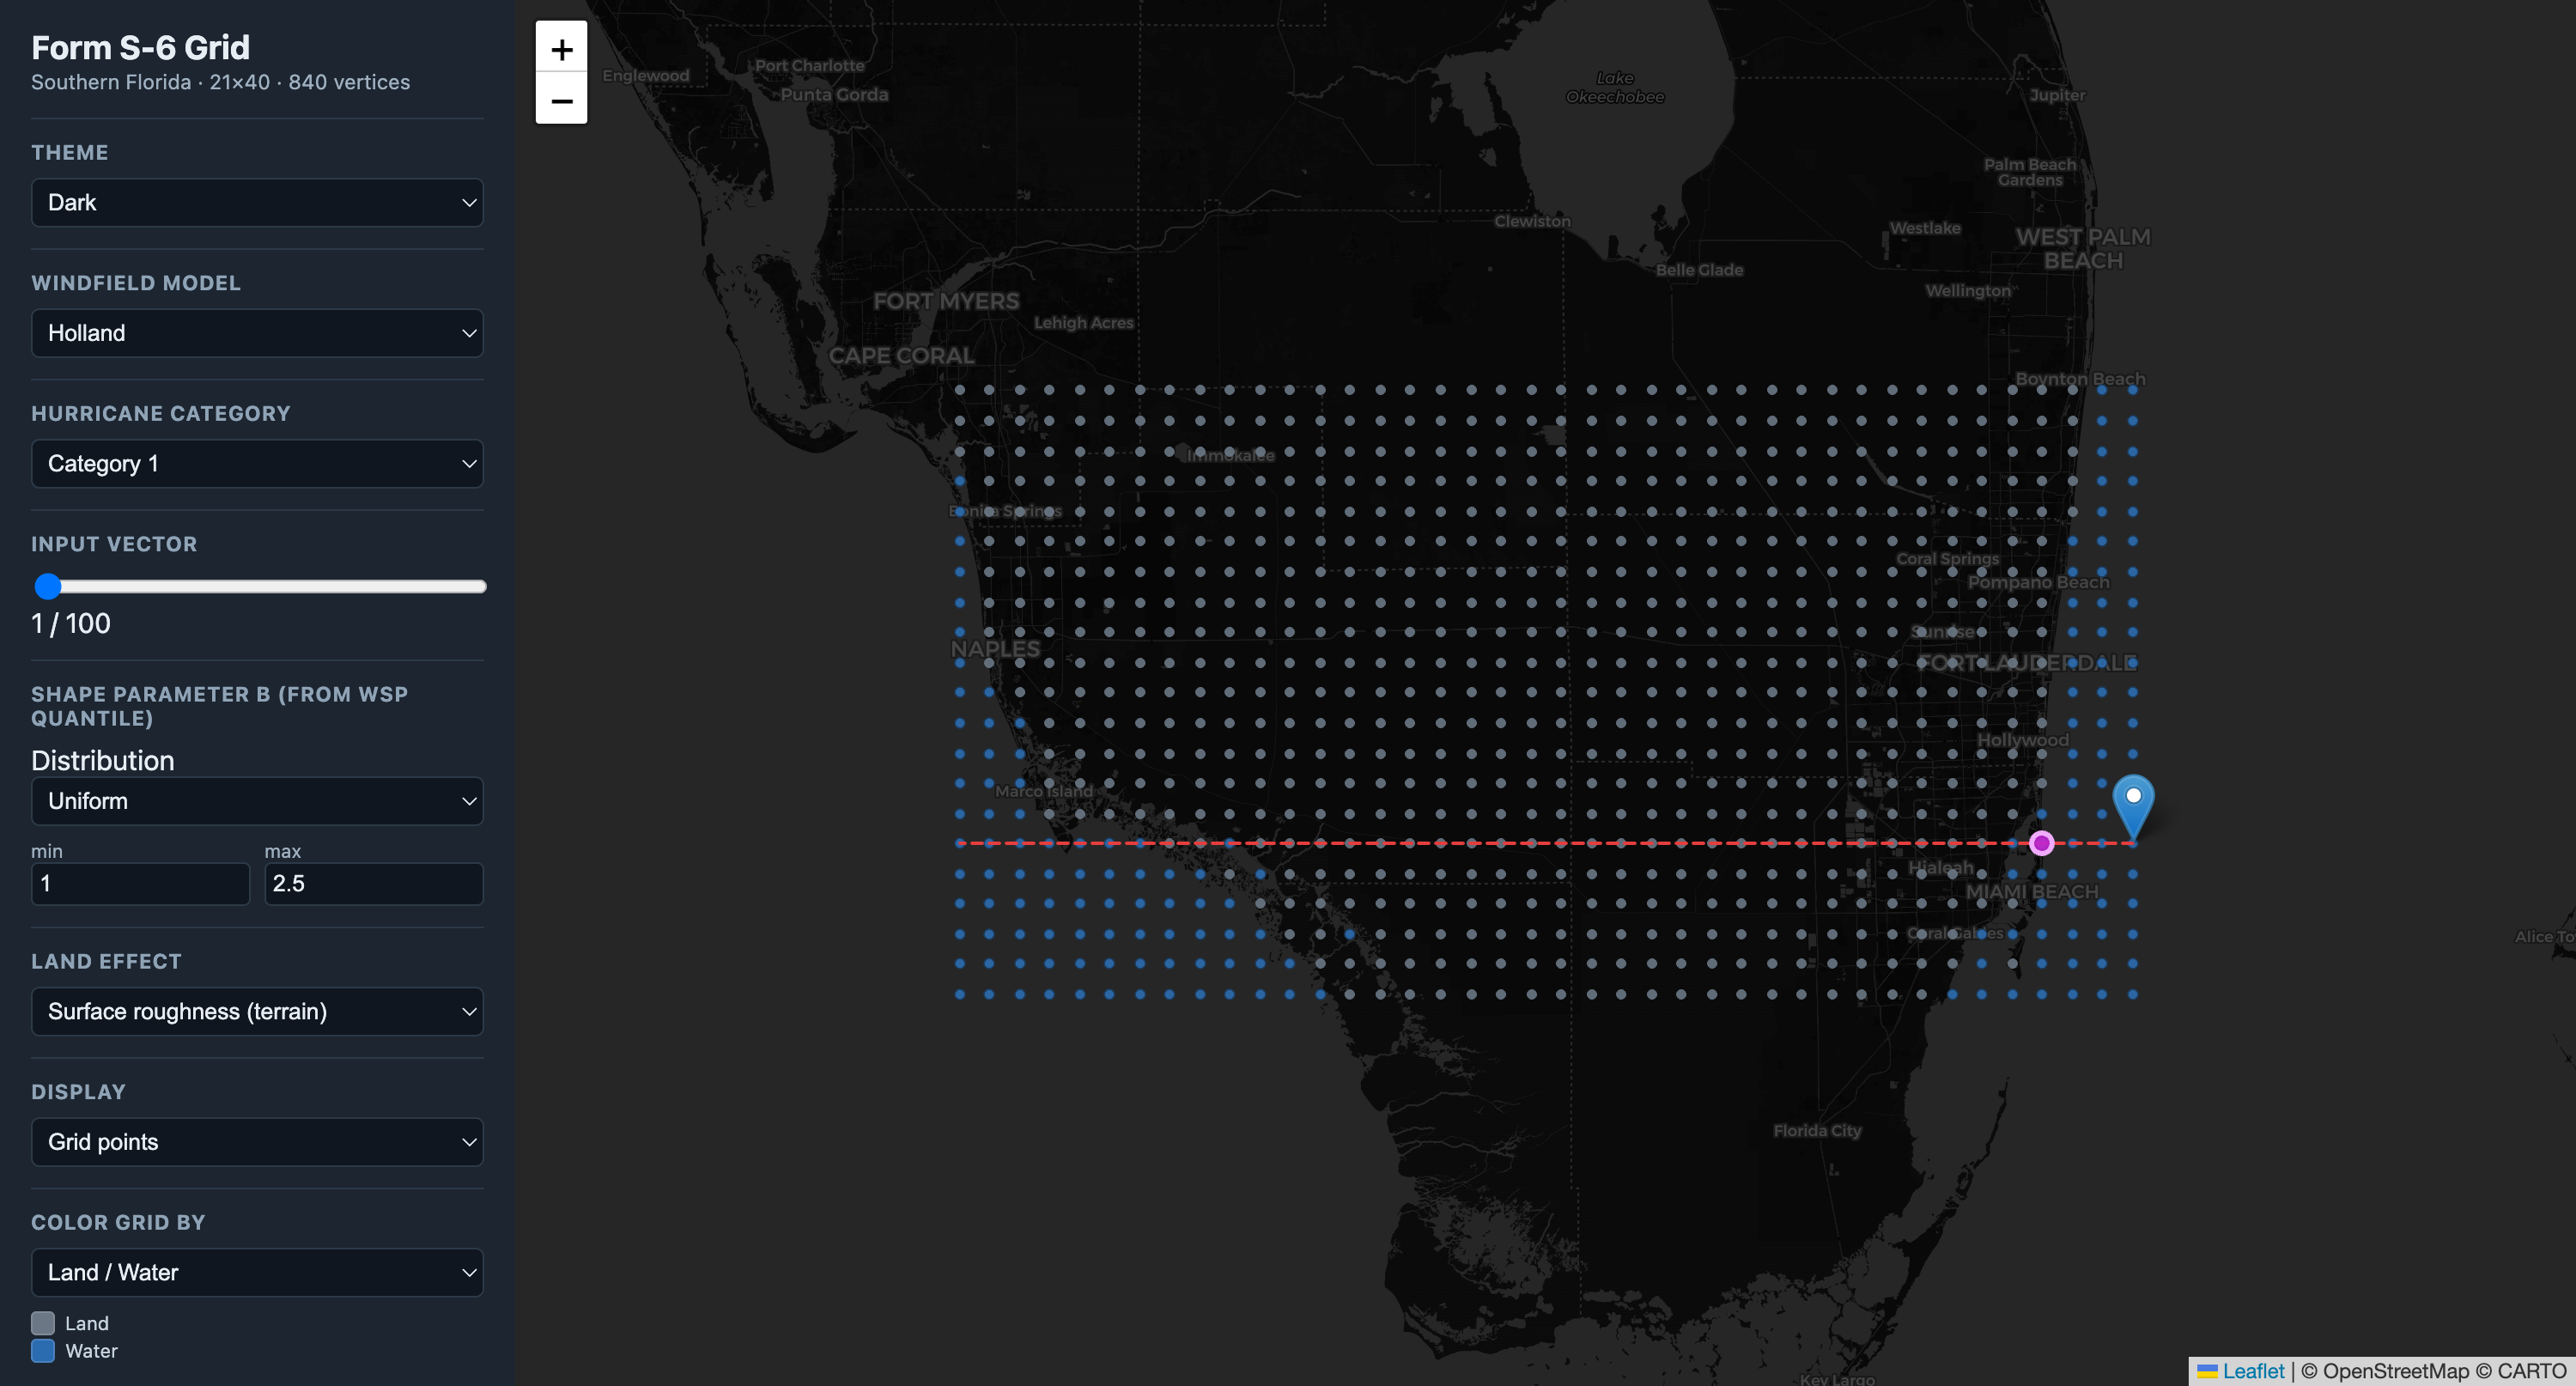
\includegraphics[width=\textwidth]{grid_basemap.png}
\caption{The 840-vertex Form S-6 grid over southern Florida: land (grey) and
water (blue) vertices, the due-west storm track (dashed), the $t\!=\!0$ centre,
and the landfall marker.}
\label{fig:grid}
\end{figure}

\section{Wind-field models}
Three wind-field models are provided, each evaluated at all 840 vertices.
\textbf{Powell} is an iterative boundary-layer PDE (slab) solver;
\textbf{Holland} is the closed-form gradient-wind profile; \textbf{Willoughby}
is a piecewise power-law profile anchored to the Holland $V_{\max}$. All three
include translation asymmetry from the storm motion. Powell is precomputed in
Python (PyTorch/MPS, $\sim$2.3\,s per solve); Holland and Willoughby are
closed-form and computed live in the browser.

Per-vector inputs come from the \texttt{SA all Variables} worksheet: central
pressure CP, radius of maximum wind Rmax, translation speed VT, wind-field shape
parameter WSP, conversion factor CF, and far-field pressure FFP, for 100 vectors
in each of categories 1, 3, and 5. The pressure deficit is $\Delta p=\text{FFP}-\text{CP}$.
WSP is supplied as a quantile $p\in[0,1]$ and mapped to the Holland shape
parameter $B$ through a user-selectable distribution (default Uniform$[1.0,2.5]$,
$B=B_{\min}+p\,(B_{\max}-B_{\min})$).

\paragraph{Conversion factor (CF).}
The ROA CF variable converts modelled gradient winds to surface winds using a
three-zone radial rule (ROA pp.~184--185): for $r<R_{\max}$,
$\text{CF}_{\text{eff}}=\text{CF}\cdot r/R_{\max}$; for
$R_{\max}\!<\!r\!<\!3R_{\max}$, $\text{CF}_{\text{eff}}=\text{CF}-0.1\,(r-R_{\max})/(2R_{\max})$;
and for $r>3R_{\max}$, $\text{CF}_{\text{eff}}=\text{CF}-0.1$. The models are run
at gradient level ($\beta_{10}=1$) and CF performs the gradient$\to$surface
conversion exactly as specified.

\paragraph{Peak-wind metric and time sampling.}
For each vector we record the per-vertex \textbf{12-hour peak surface wind}. The
storm position is sampled finely ($\Delta t=0.1$\,h); coarse hourly sampling
aliases the fast westward motion and produces a spurious ``comb'' artifact in the
peak field, which fine sampling removes. Figures~\ref{fig:powellpts} and
\ref{fig:contours} show the peak field as coloured points and as filled contours.

\begin{figure}[H]
\centering
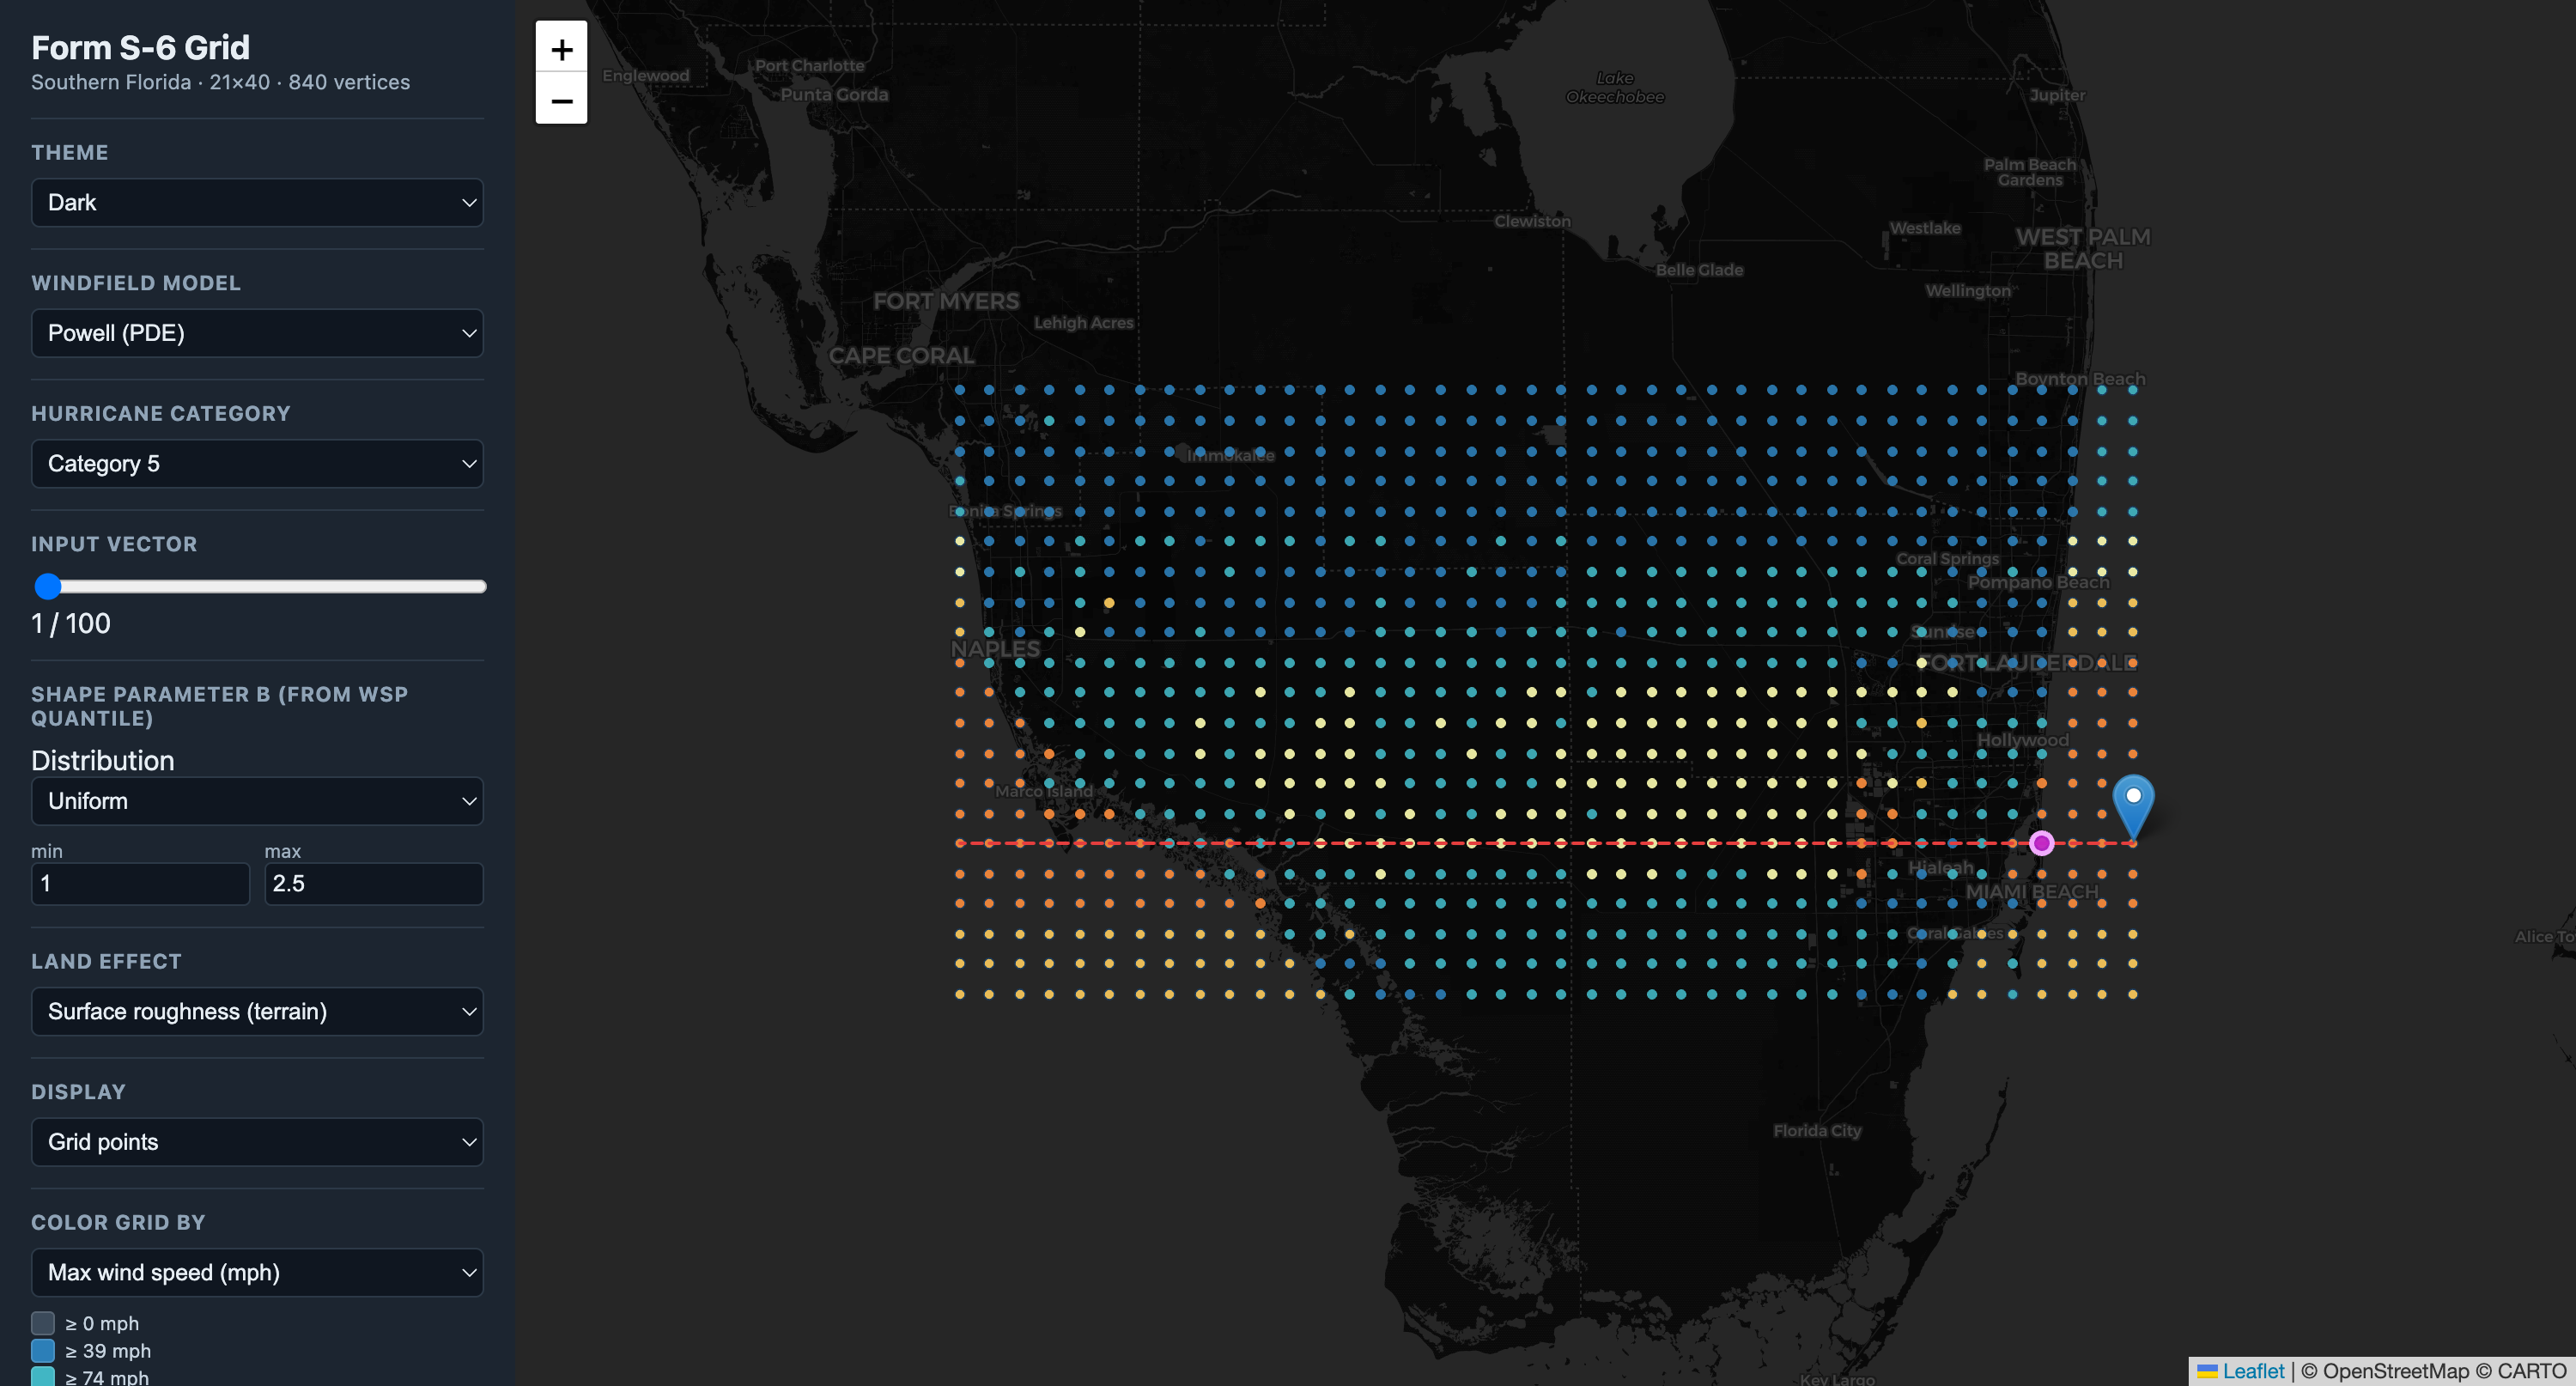
\includegraphics[width=\textwidth]{powell_cat5_pts.png}
\caption{Powell peak surface wind (Category 5, vector 1) coloured per vertex,
with surface roughness applied. Strongest winds lie north of the track---correct
for a westward-moving Northern-Hemisphere cyclone, where translation adds to
rotation on the north side.}
\label{fig:powellpts}
\end{figure}

\begin{figure}[H]
\centering
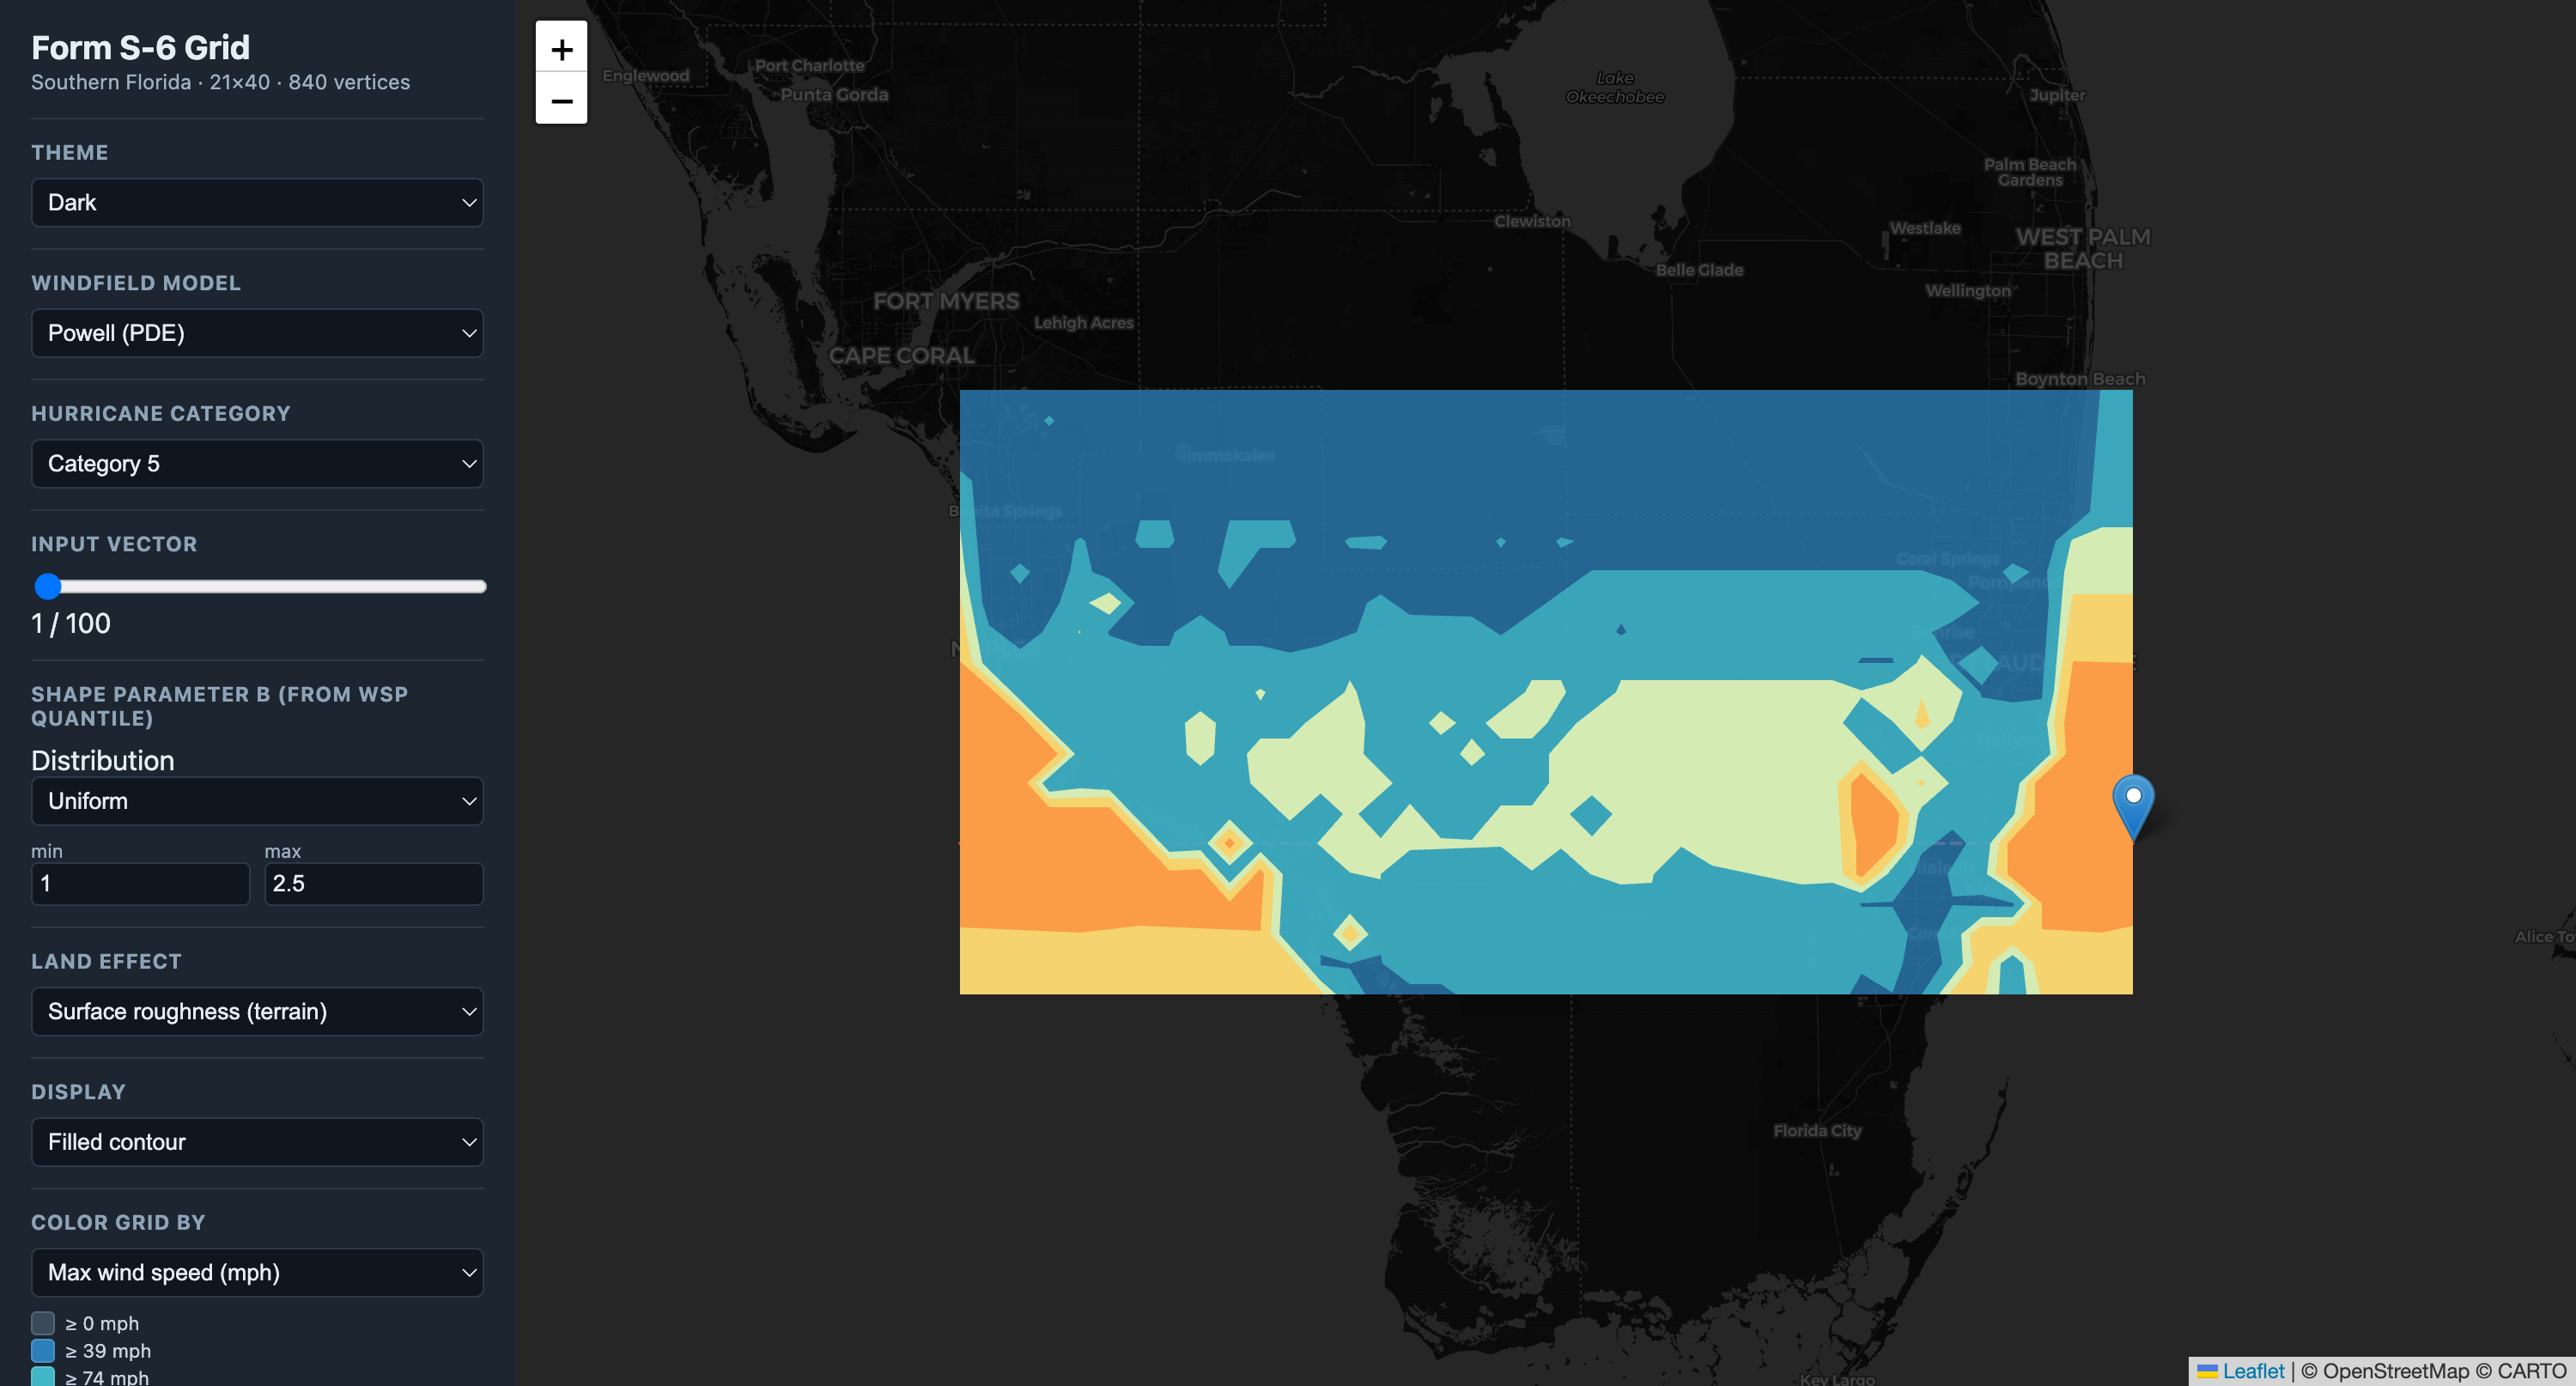
\includegraphics[width=0.49\textwidth]{powell_cat5_contour.png}\hfill
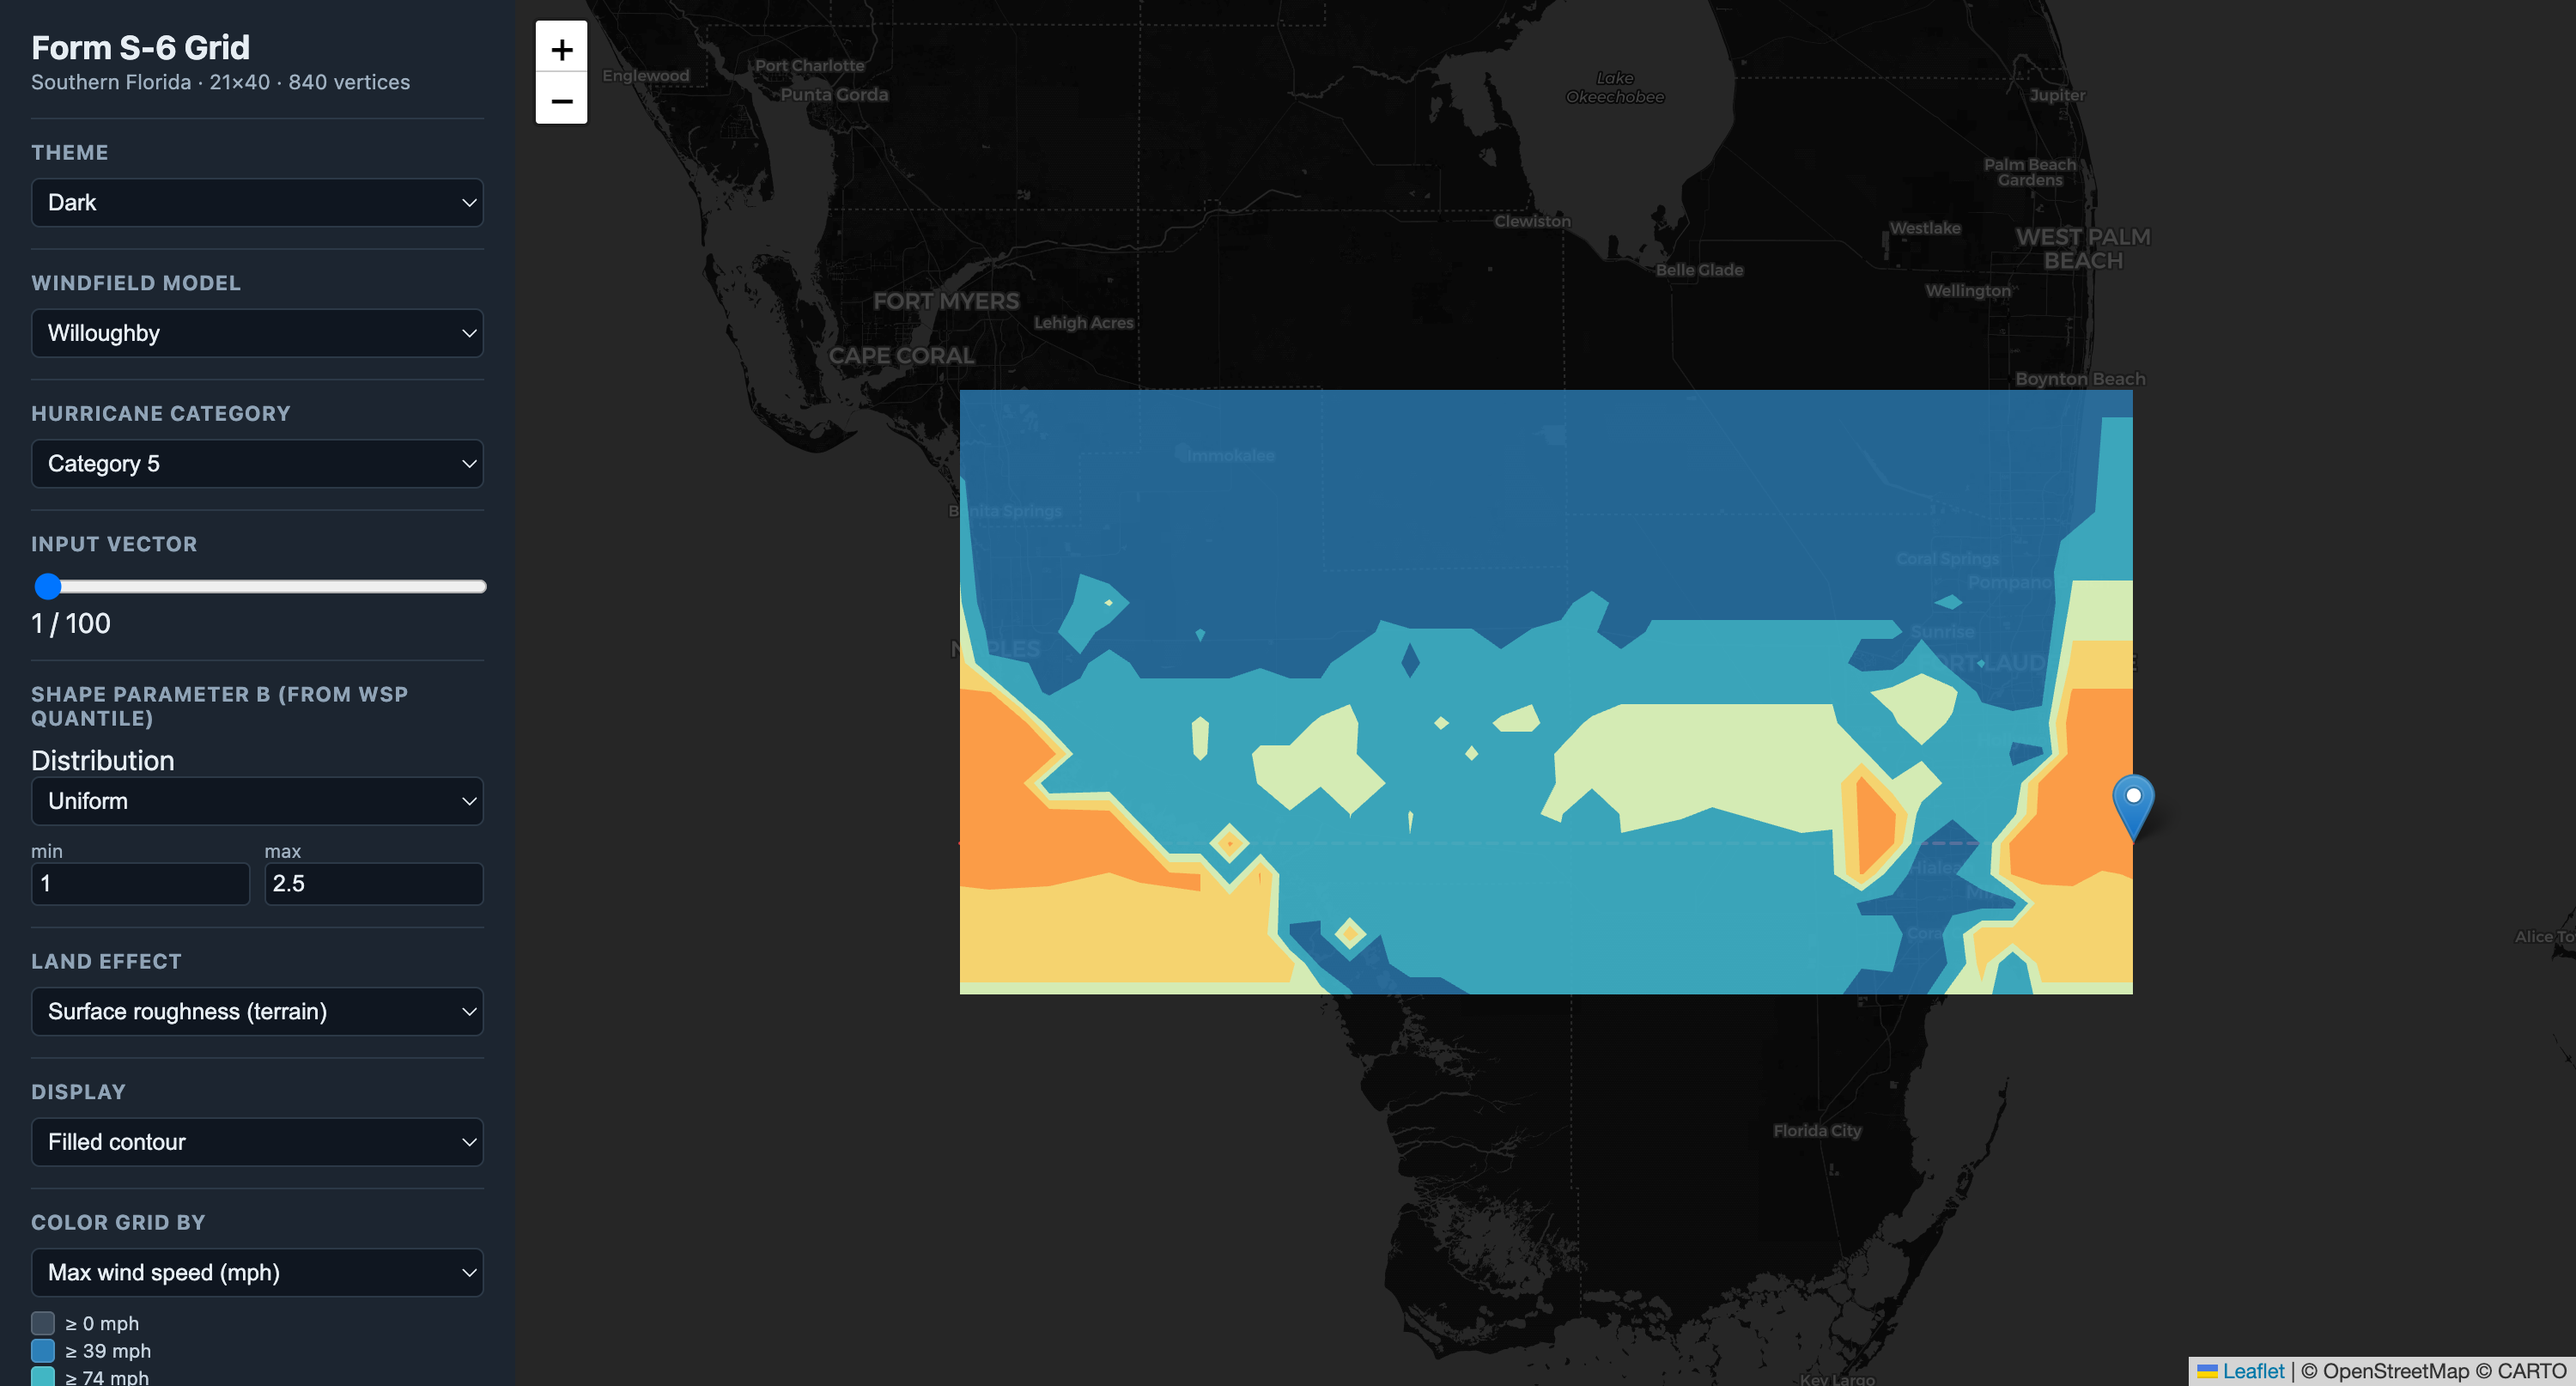
\includegraphics[width=0.49\textwidth]{willoughby_cat5_contour.png}
\caption{Filled-contour display (ROA Figs.~6--8 style) of the Category 5 peak
field: Powell (left) and Willoughby (right). Contours are built on the $21\times40$
lattice with the wind-speed colour bands.}
\label{fig:contours}
\end{figure}

\section{Land effect: roughness and decay}
A single \emph{land-effect} selector offers three mutually exclusive treatments
of the storm's interaction with the land: \textbf{None} (marine winds),
\textbf{Surface roughness}, and \textbf{Kaplan--DeMaria decay}.

\paragraph{Surface roughness.}
Roughness is applied as a per-vertex, wind-speed-independent multiplier on the
final surface wind. The roughness length $z_0$ at each vertex is sampled from
\textbf{NLCD~2021 land cover} (fetched as a properly georeferenced GeoTIFF from
the MRLC WCS) via a published land-cover$\to z_0$ table, then converted from
marine to terrain exposure with the gradient-tied \textbf{log-law}
(Vickery et al.\ 2009 / ESDU):
\[
\text{factor}=\frac{\ln(z_{\text{ref}}/z_{0,\text{land}})/\ln(z_g/z_{0,\text{land}})}
{\ln(z_{\text{ref}}/z_{0,\text{marine}})/\ln(z_g/z_{0,\text{marine}})},
\]
with $z_{\text{ref}}=10$\,m and gradient height $z_g=500$\,m; water returns
$\approx1$. The land-mean factor is $\approx0.67$ (urban $\sim0.50$, wetland
$\sim0.70$). This is a \emph{spatial} terrain-friction effect.

\paragraph{Kaplan--DeMaria decay.}
Roughness alone cannot reproduce a storm weakening as it moves inland, which is
a \emph{temporal} filling process. The Kaplan--DeMaria (1995) model is offered as
a separate option: a one-time coastal reduction ($R=0.90$) at first landfall, then
$V(t)=V_b+(R\,V_0-V_b)\,e^{-\alpha t}$ with $\alpha=0.095\,\text{h}^{-1}$ and
background $V_b=30.7$\,mph over land, with a gentle recovery
($\alpha_{\text{rec}}=0.05\,\text{h}^{-1}$) once the centre re-emerges over the
Gulf. Landfall ($\approx$E-W~9) and Gulf exit ($\approx$E-W~99) are read from the
$N$-$S=0$ track land mask. Figure~\ref{fig:kdloss}~(left) shows the resulting
inland decay for a Category~5 storm. The two options are kept exclusive because
$\alpha$ already lumps surface friction with loss of the ocean energy source.

\section{Sensitivity and uncertainty analysis}
Following Iman, Johnson, and Schroeder (2001), as the ROA cites:
\begin{itemize}
\item \textbf{Sensitivity (SRC).} Standardized regression coefficients from
regressing the standardized output on the six standardized inputs over the 100
SA vectors, per category. Sign gives direction, magnitude gives influence
(ROA Fig.~9).
\item \textbf{Uncertainty (EPR).} Expected percentage reduction in output
variance per input (ROA Fig.~10). For \emph{Powell} the EPR is the variance share
\[
\text{EPR}_i=\frac{\mathrm{Var}\!\left(Y\,\middle|\,\text{only }X_i\text{ varies}\right)}
{\mathrm{Var}(Y_{\text{SA}})}\times100\%,
\]
computed faithfully from the six one-variable ROA ``UA for $X$'' worksheets
(1{,}800 PDE solves); the analytic models use the
$\text{EPR}_i=\text{SRC}_i^2$ approximation.
\end{itemize}
The output metric is the \textbf{mean peak wind over the 682 land vertices}
(loss-cost is the additional metric in Section~\ref{sec:loss}). The computed
SRCs and faithful EPRs reproduce the ROA's findings: WSP dominates for
Category~1 while Rmax grows to dominate for Category~5 (faithful EPR: Cat~1
WSP~$\approx54\%$, Cat~5 Rmax~$\approx57\%$), with CP negative and CF, FFP, Rmax
positive (Figure~\ref{fig:analysis}).

\begin{figure}[H]
\centering
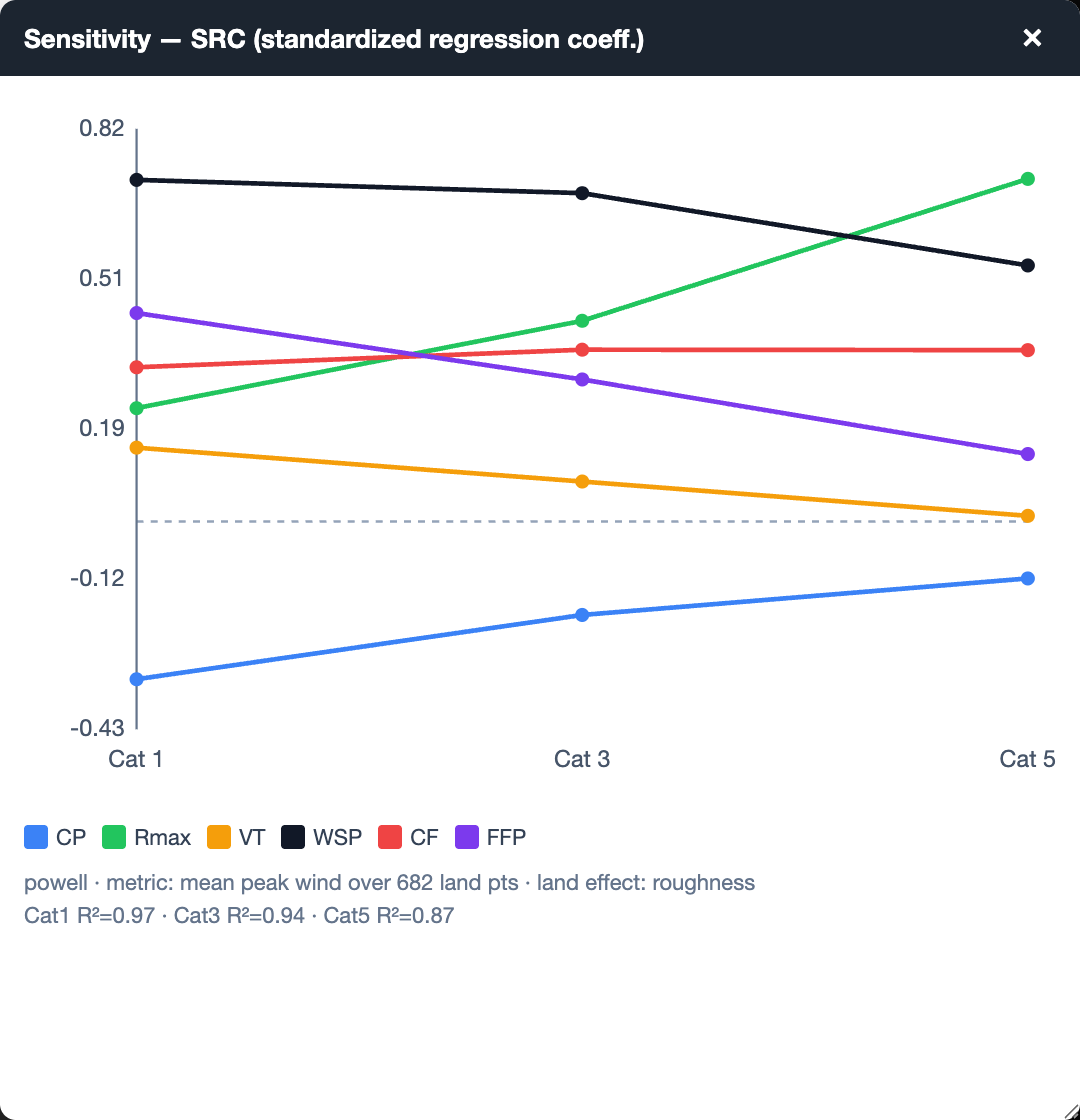
\includegraphics[width=0.49\textwidth]{analysis_src.png}\hfill
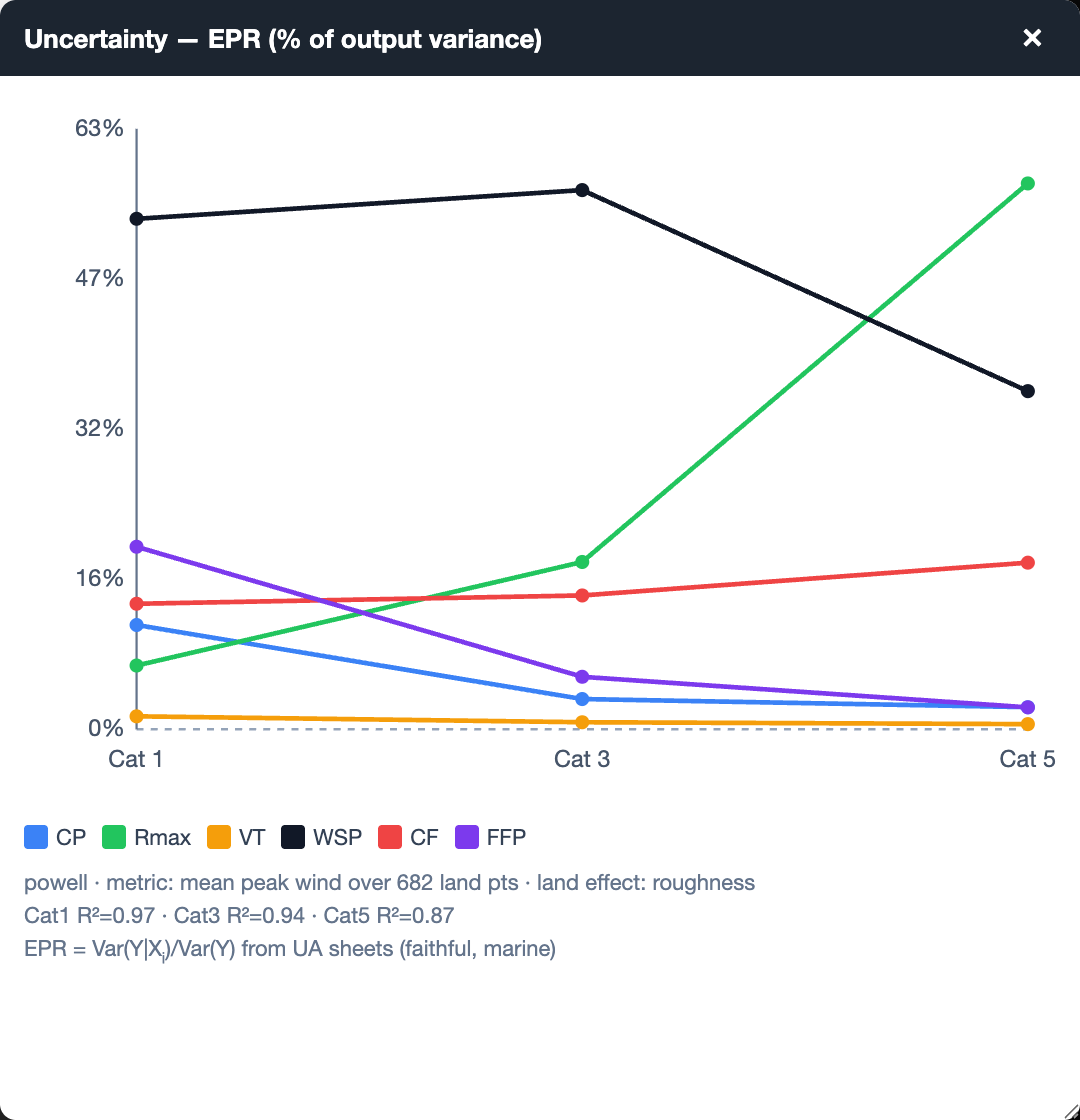
\includegraphics[width=0.49\textwidth]{analysis_epr.png}
\caption{Sensitivity (SRC, left) and uncertainty (EPR, right) for the Powell
model, plotted by hurricane category---the interactive analogues of ROA
Figs.~9--10. The windows are independently movable and resizable.}
\label{fig:analysis}
\end{figure}

\section{Vulnerability and loss cost}\label{sec:loss}
The ROA (p.~186) fixes a single insured structure at \emph{every} one of the 682
land vertices: a \$100{,}000, zero-deductible, single-family, single-story,
masonry, gable-roof, no-shutter home with truss anchors, shingles over 15\# felt,
a $\tfrac12$\,in.\ plywood deck (8d nails at 6\,in.\ edge / 12\,in.\ field), built
1995, roof age unknown. Because the structure is uniform, a \textbf{single
vulnerability curve} applies at all points and only the wind varies.

The curve is generated from our existing HAZUS/ARA wind-vulnerability tool
(\texttt{wind\_\allowbreak vulnerability\_\allowbreak tool\_\allowbreak v5.html})
driven headlessly to the structure
above, yielding Mean Damage Ratio (MDR) versus the ASCE~7-98 3-second peak gust at
10\,m (Exposure~C). The resulting masonry curve (Figure~\ref{fig:vuln}) is a smooth
sigmoid: $\sim$0 below 50\,mph, 50\% near 100\,mph, and a plateau at MDR~$\approx
0.60$ above $\sim$140\,mph---the masonry ceiling (walls survive; roof, openings,
and contents bound the loss), in contrast to frame construction which approaches
1.0.

\begin{figure}[H]
\centering
\includegraphics[width=0.7\textwidth]{vulnerability_curve.png}
\caption{Form S-6 vulnerability curve (Mean Damage Ratio vs.\ peak 3-second gust)
for the masonry, gable, no-shutter structure, generated from the HAZUS/ARA tool.}
\label{fig:vuln}
\end{figure}

Per-vertex loss is $\text{loss}=\text{MDR}(\text{peak wind})\times\$100{,}000$;
the expected loss as a percent of exposure is the total over the 682 land vertices
divided by $\$68{,}200{,}000$ ($=682\times\$100{,}000$). The viewer colours the
grid by MDR, reports total loss (\$M) and \% exposure, and the hover popup shows
loss \% and dollars beside the peak wind. Figure~\ref{fig:kdloss} shows Category~5
Kaplan--DeMaria-decayed wind (left) and the corresponding loss field (right).

\begin{figure}[H]
\centering
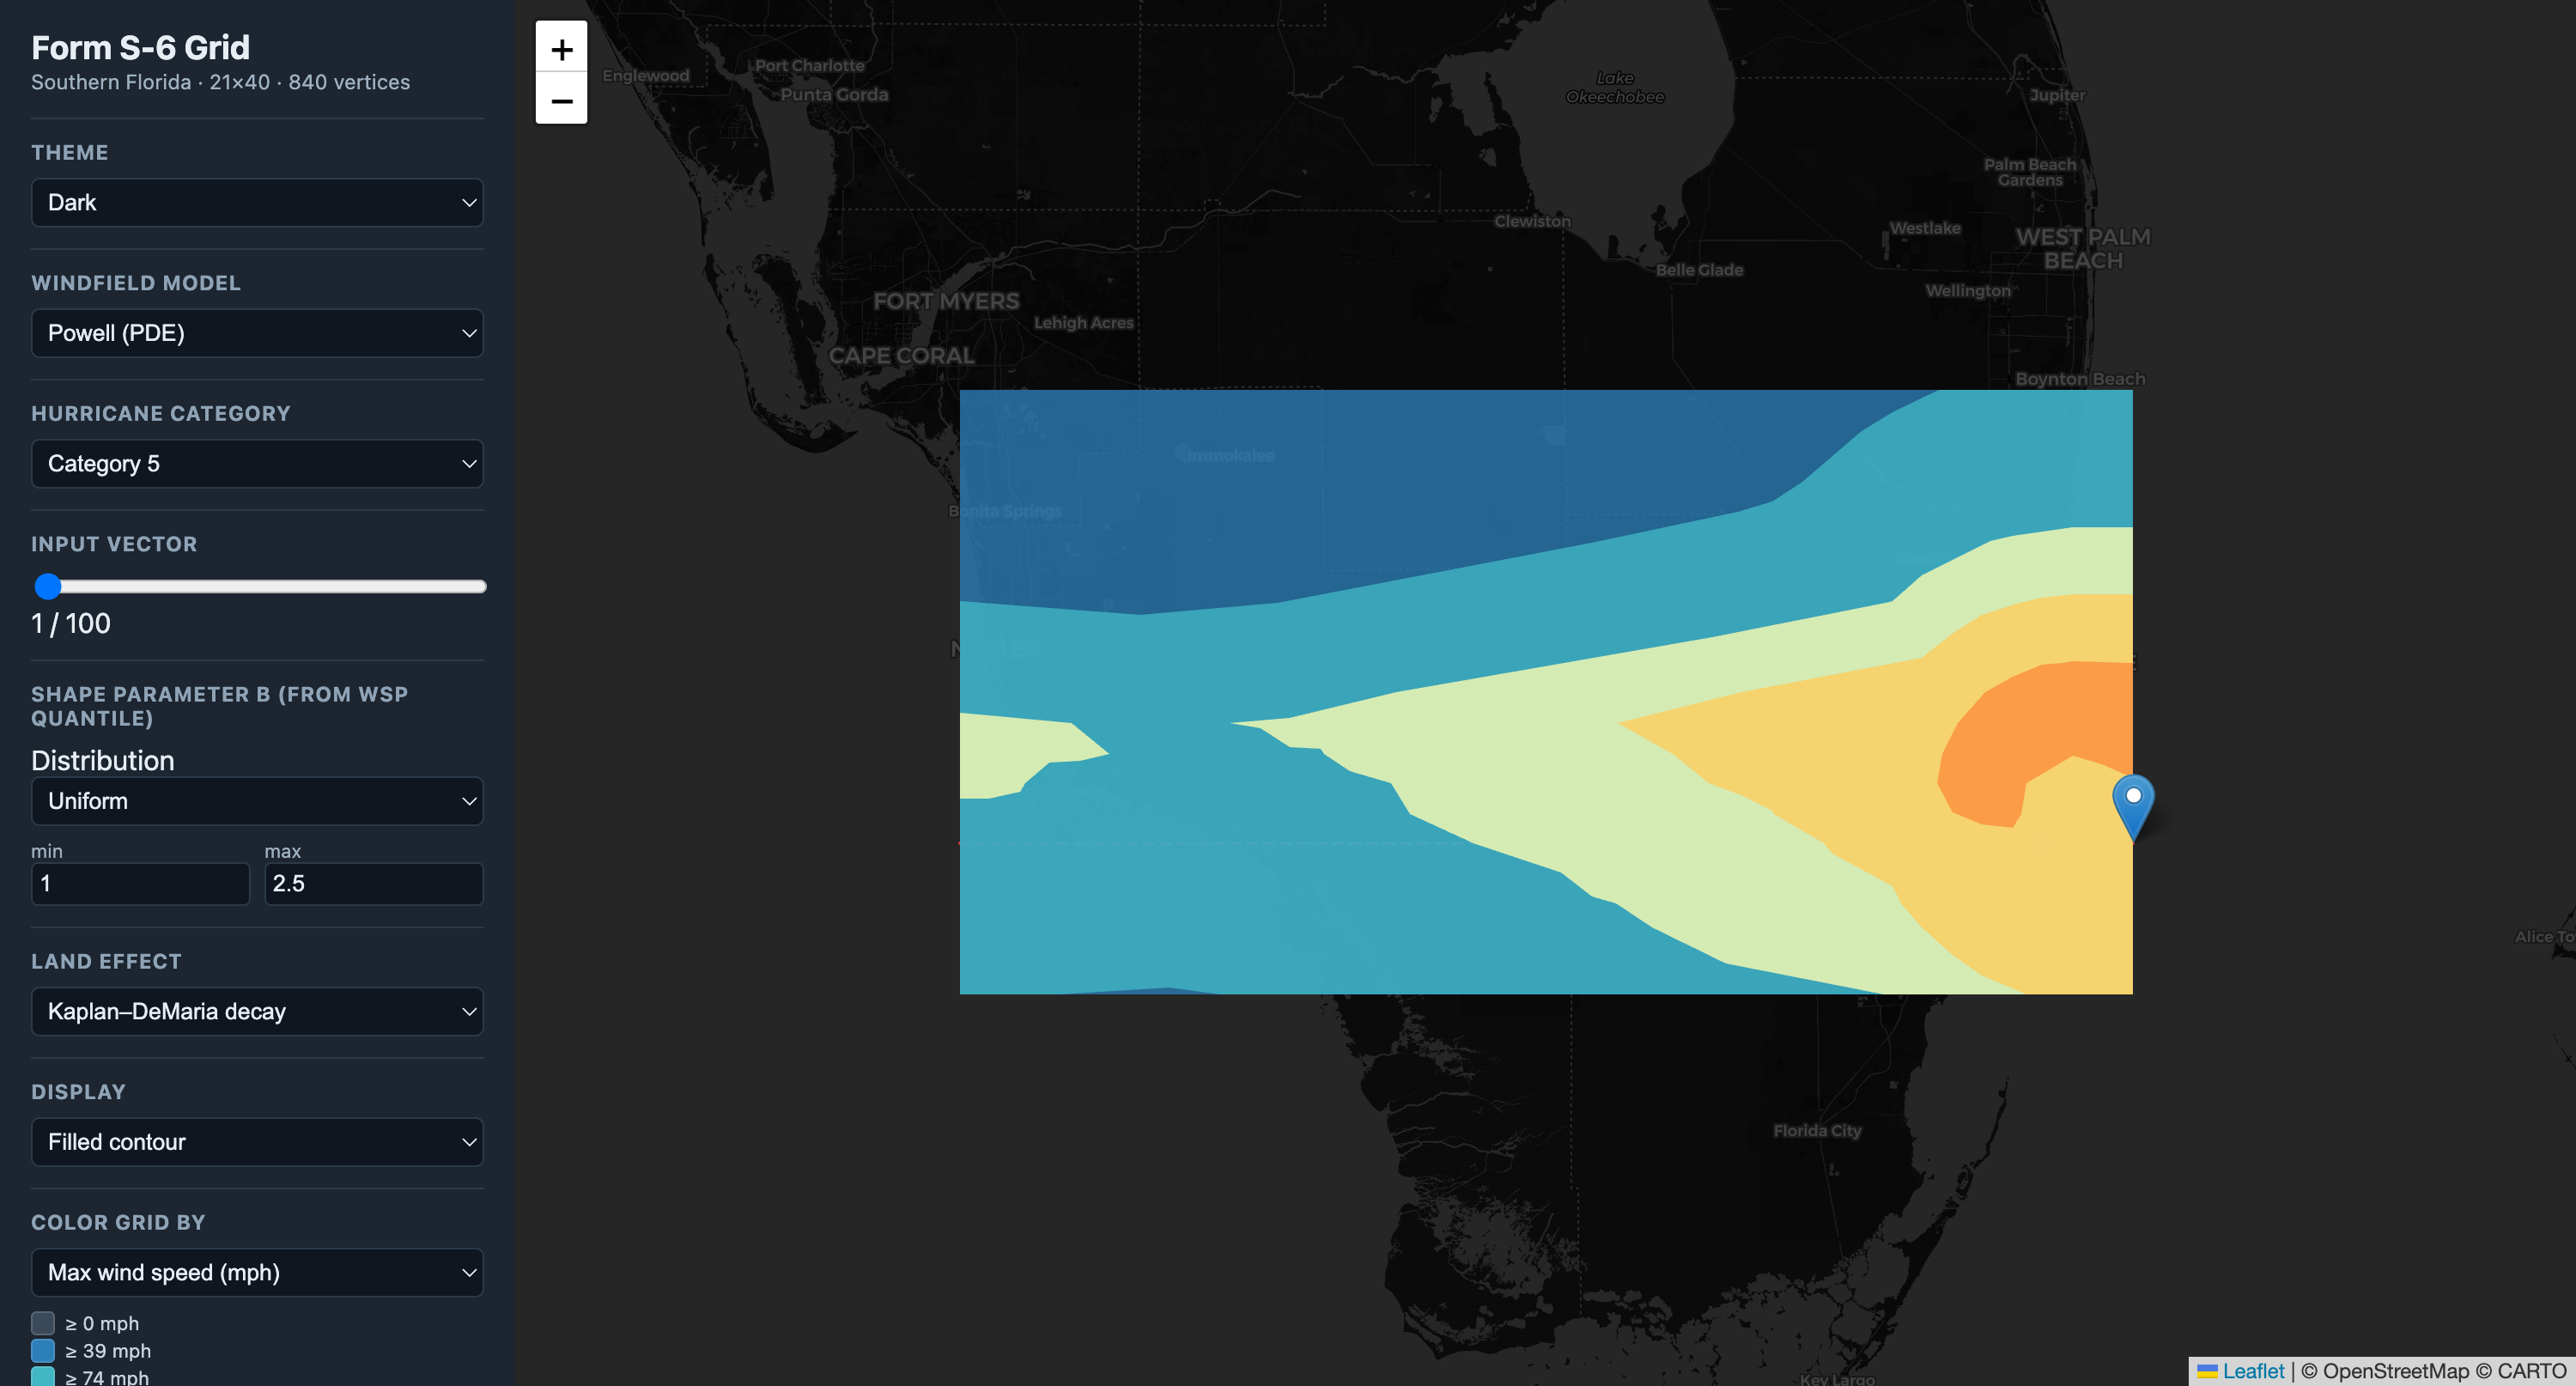
\includegraphics[width=0.49\textwidth]{powell_cat5_kd.png}\hfill
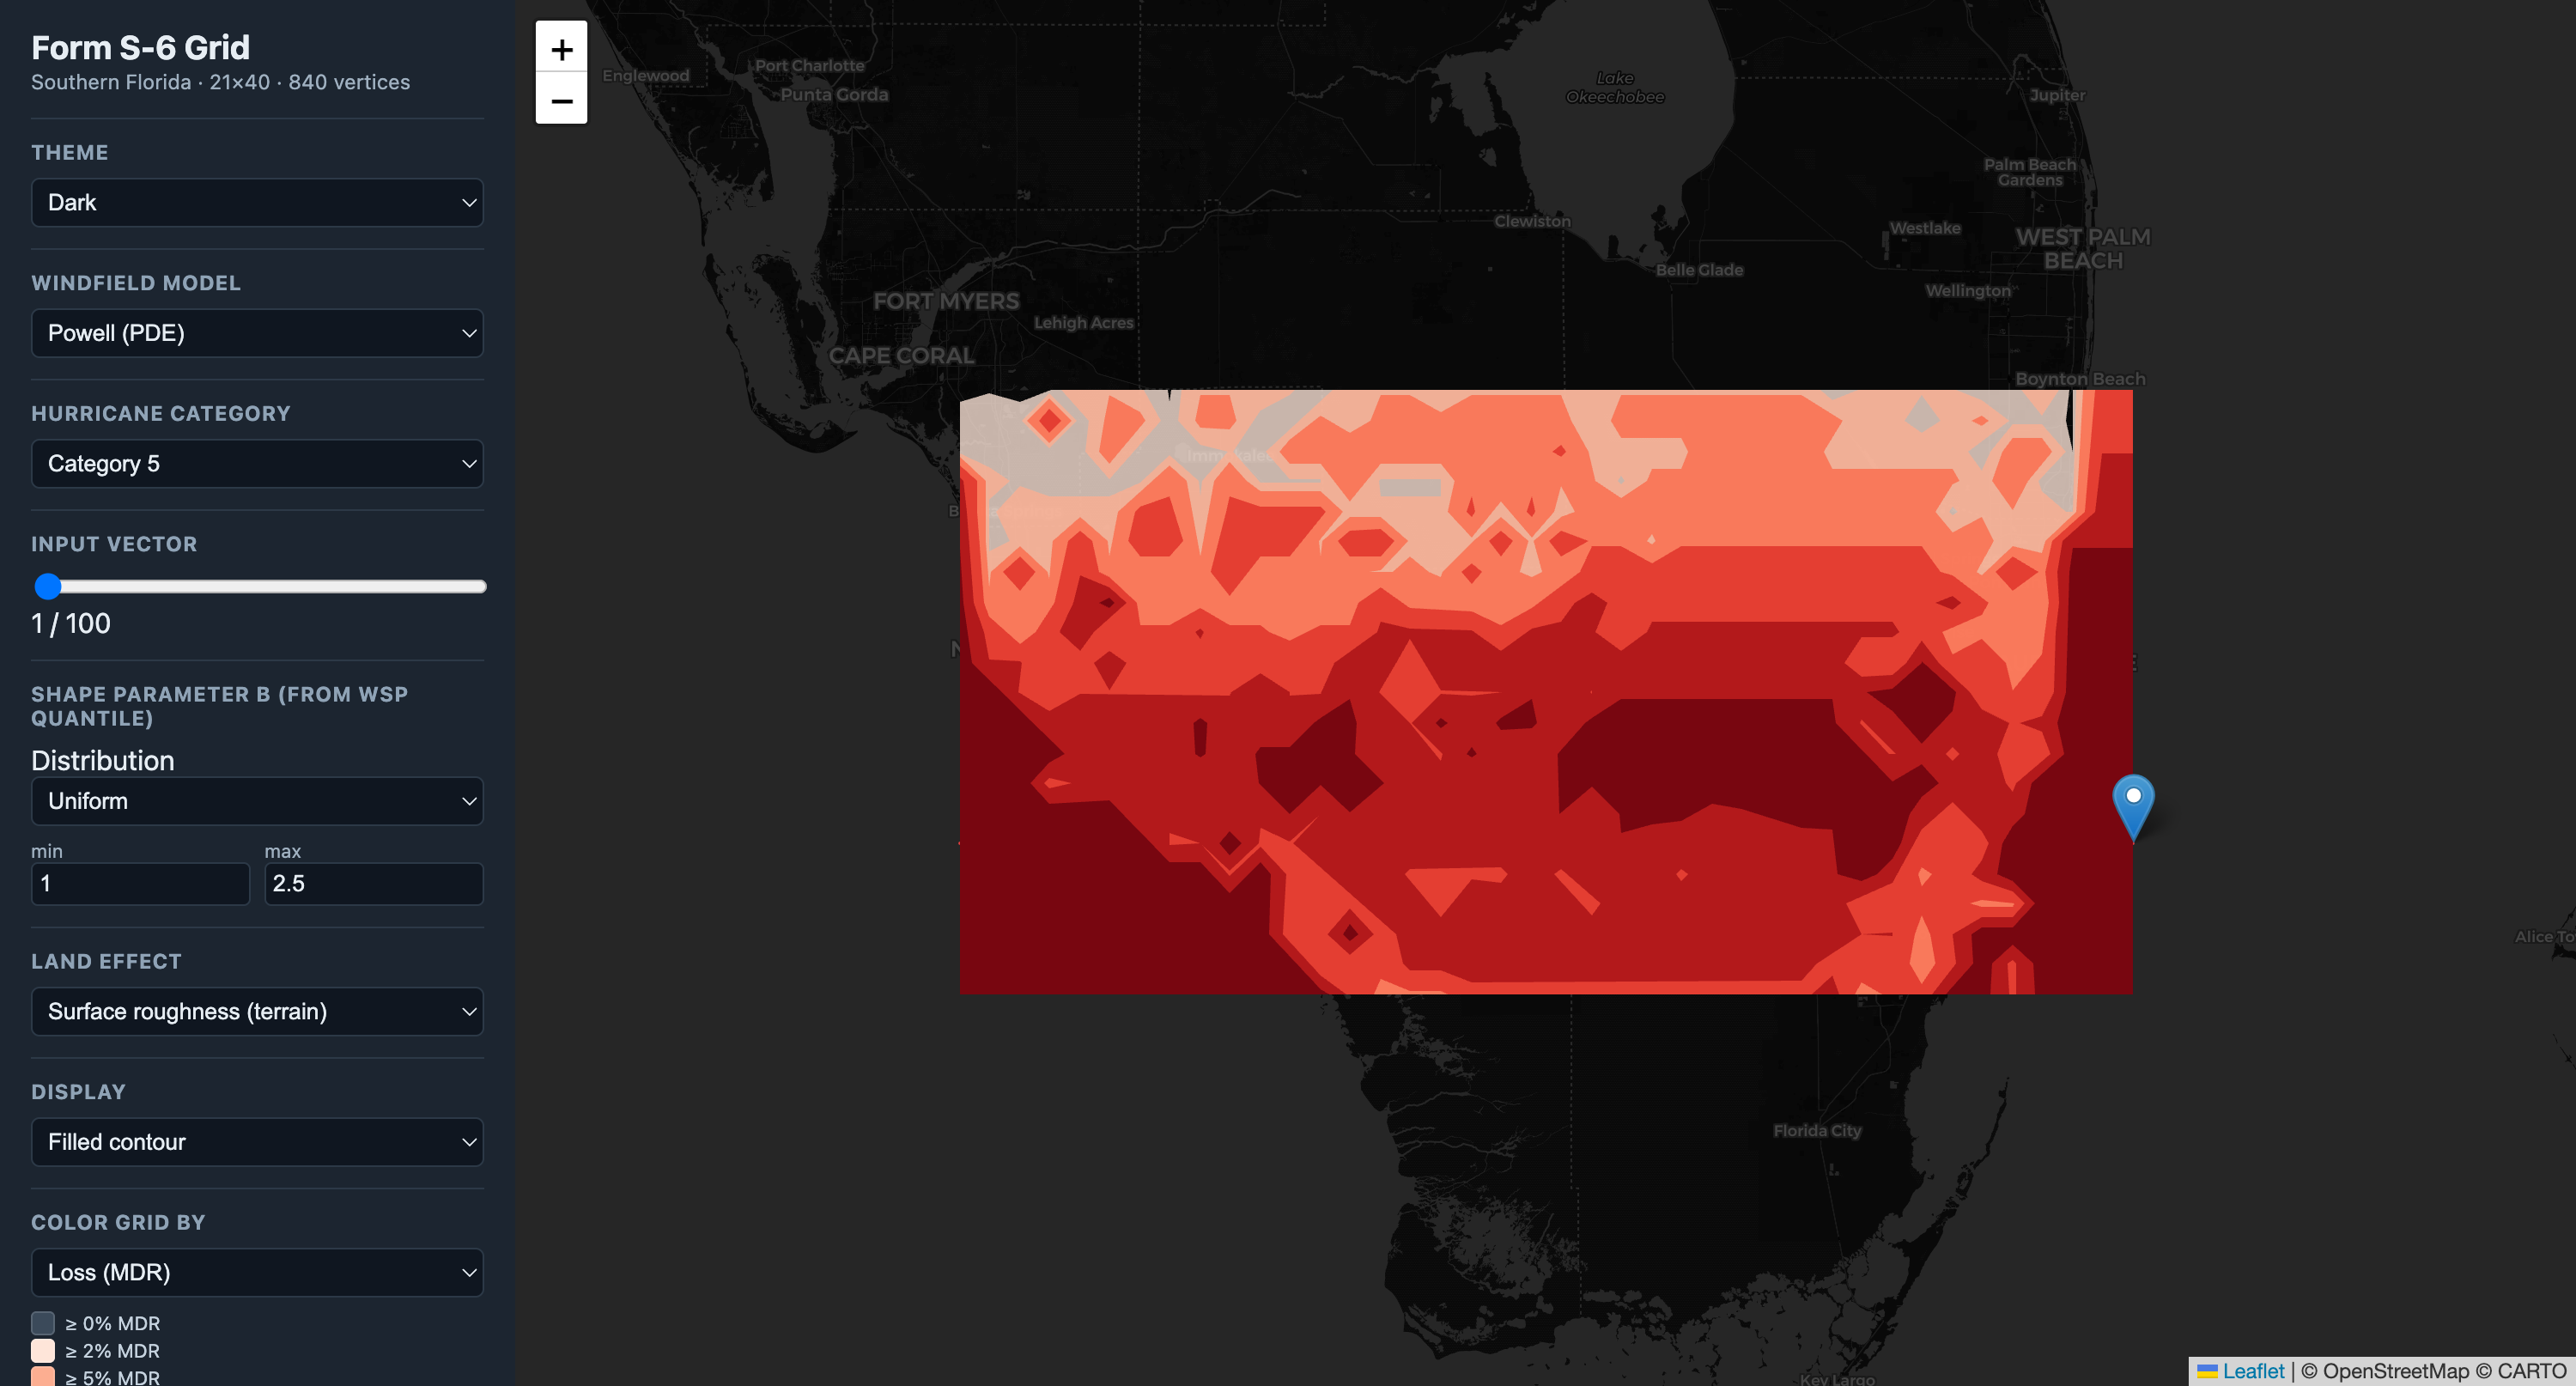
\includegraphics[width=0.49\textwidth]{powell_cat5_loss.png}
\caption{Category~5, Powell: Kaplan--DeMaria-decayed peak wind (left) and the
loss field as Mean Damage Ratio (right), both as filled contours.}
\label{fig:kdloss}
\end{figure}

\section{Interface and reproducibility}
The viewer offers model / category / input-vector selection (the input vector
chooses one of the 100 randomized storms for the category), the WSP$\to B$
distribution control, the three-way land-effect selector, a colour-by control
(peak wind, loss MDR, or land/water), a points/filled-contour display toggle,
light and dark themes (Figure~\ref{fig:light}), and nearest-point hover (peak
wind, loss, coordinates, land/water, place name, and the active input
parameters). \textbf{Left-clicking} a vertex opens a floating windfield popup
(Figure~\ref{fig:popup}) with the storm-relative isotach field---the marked
vertex at its peak time---and that vertex's wind time series over the 12-hour
passage. The Sensitivity and Uncertainty results open as independent, movable,
resizable windows.

\begin{figure}[H]
\centering
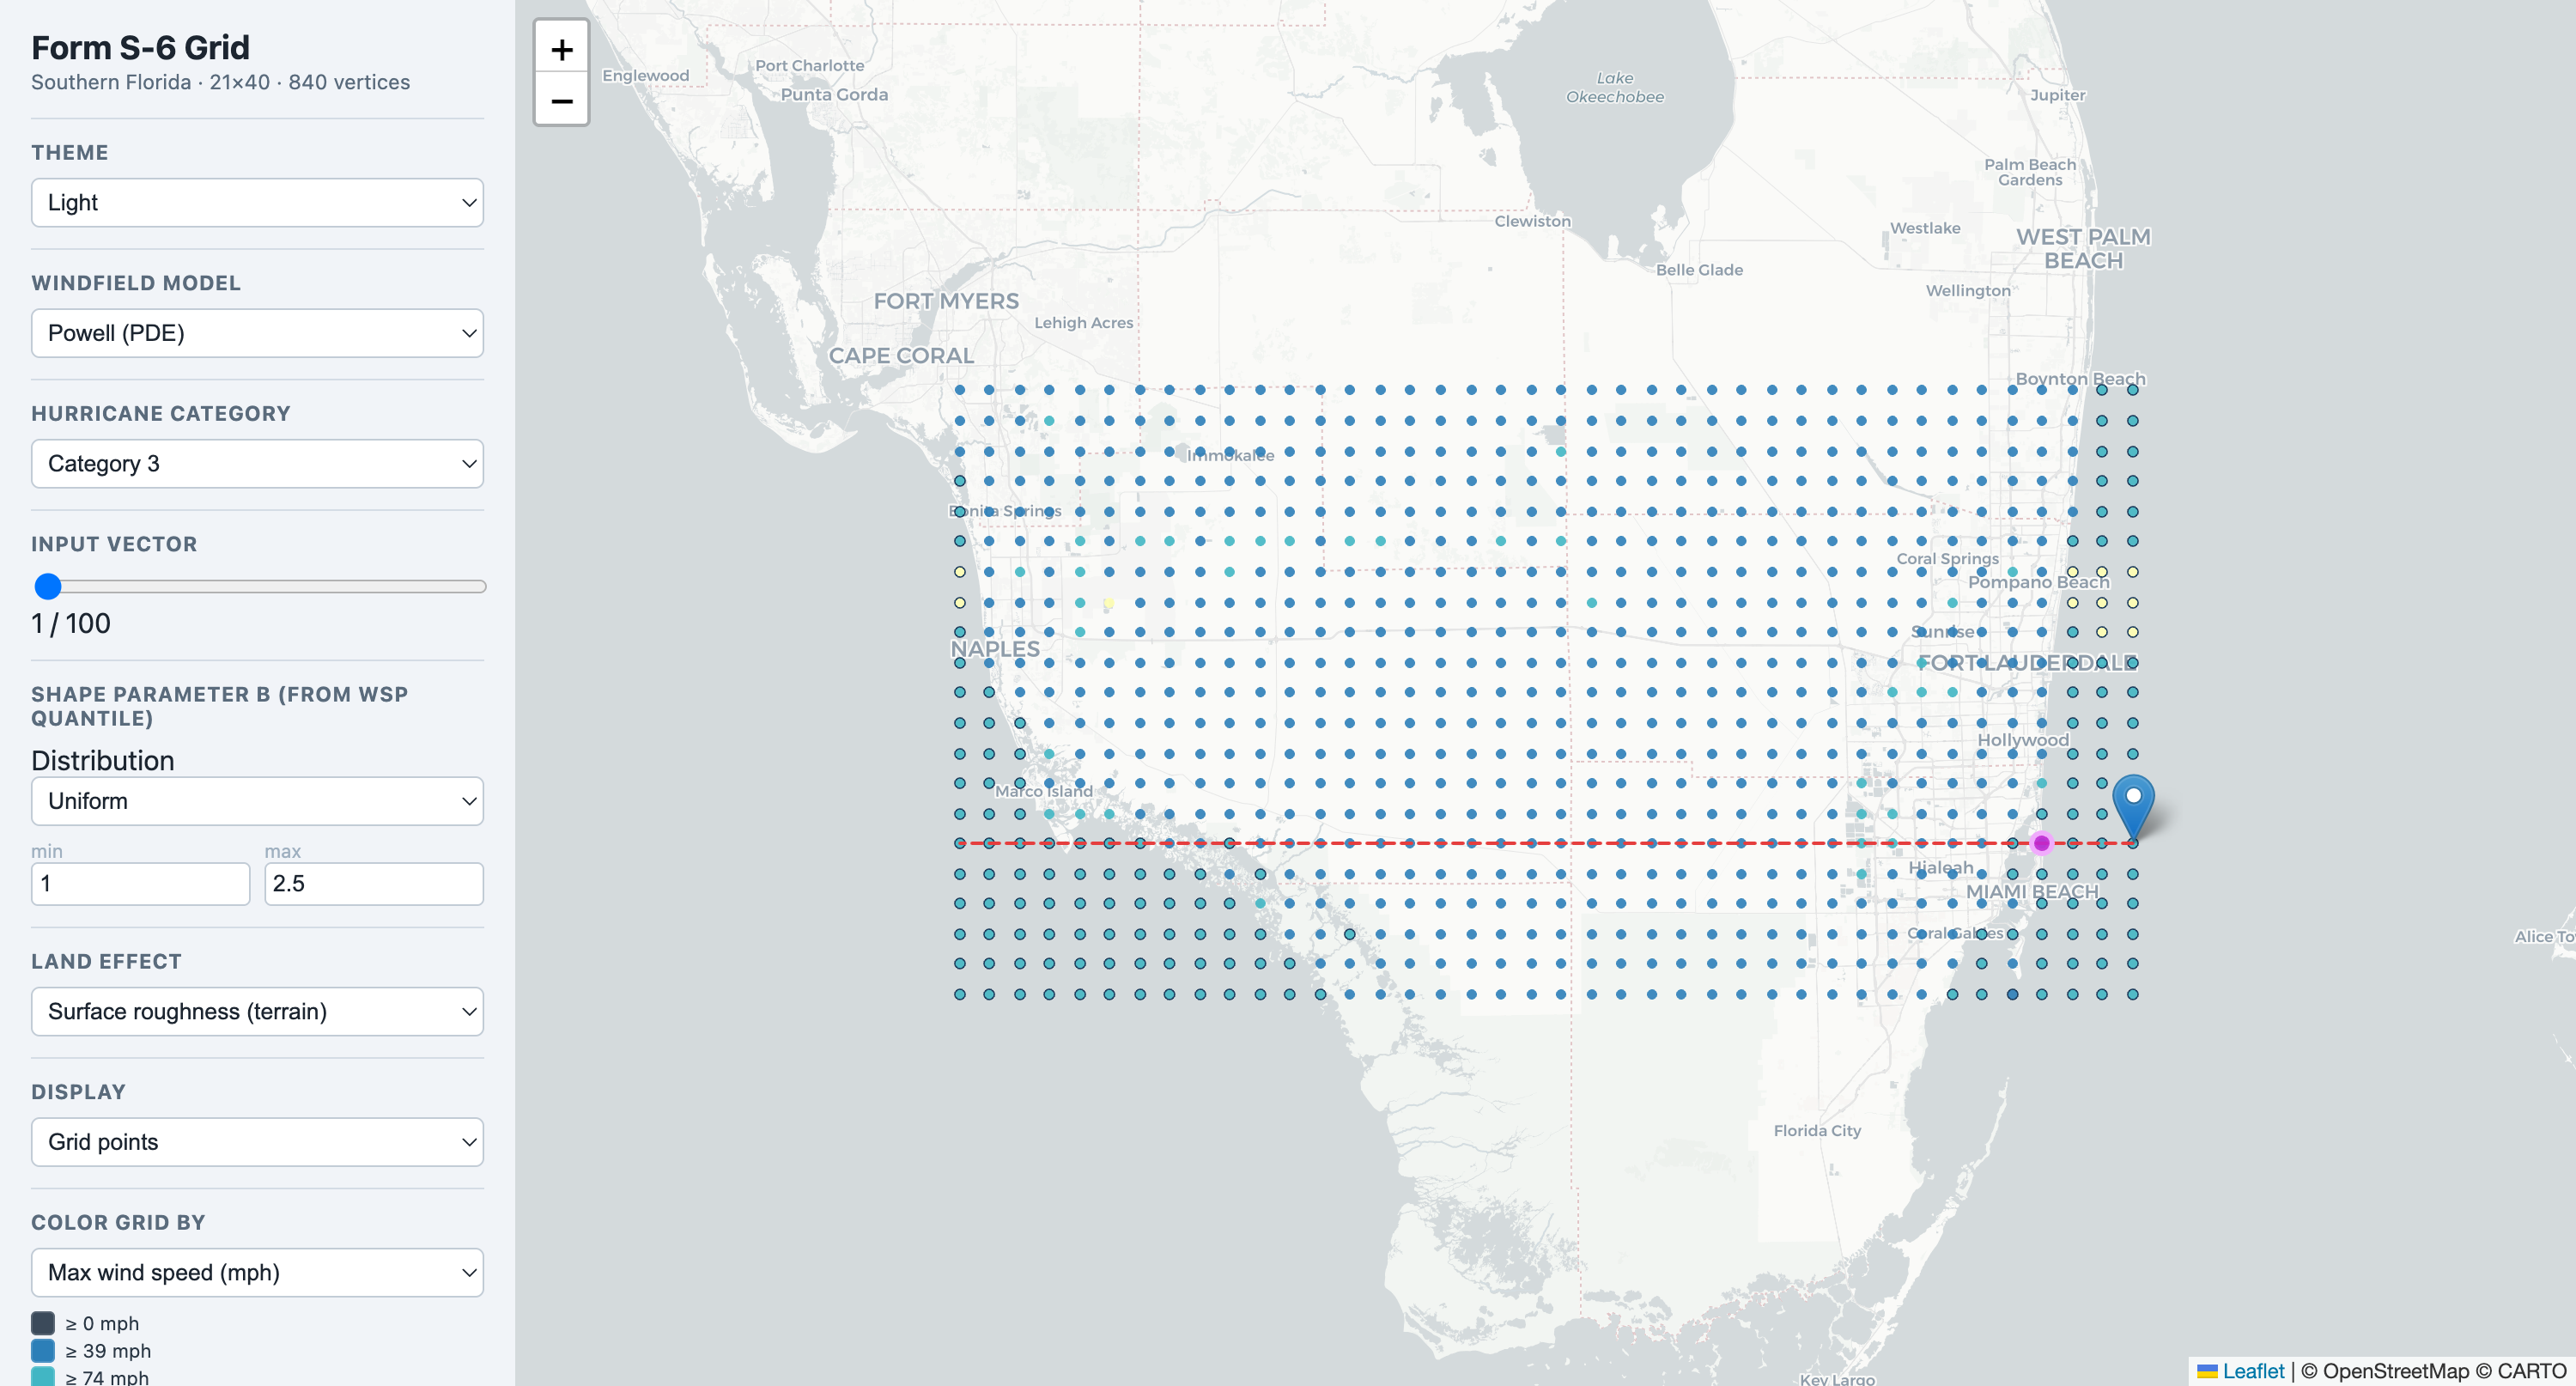
\includegraphics[width=0.46\textwidth]{light_theme.png}\hfill
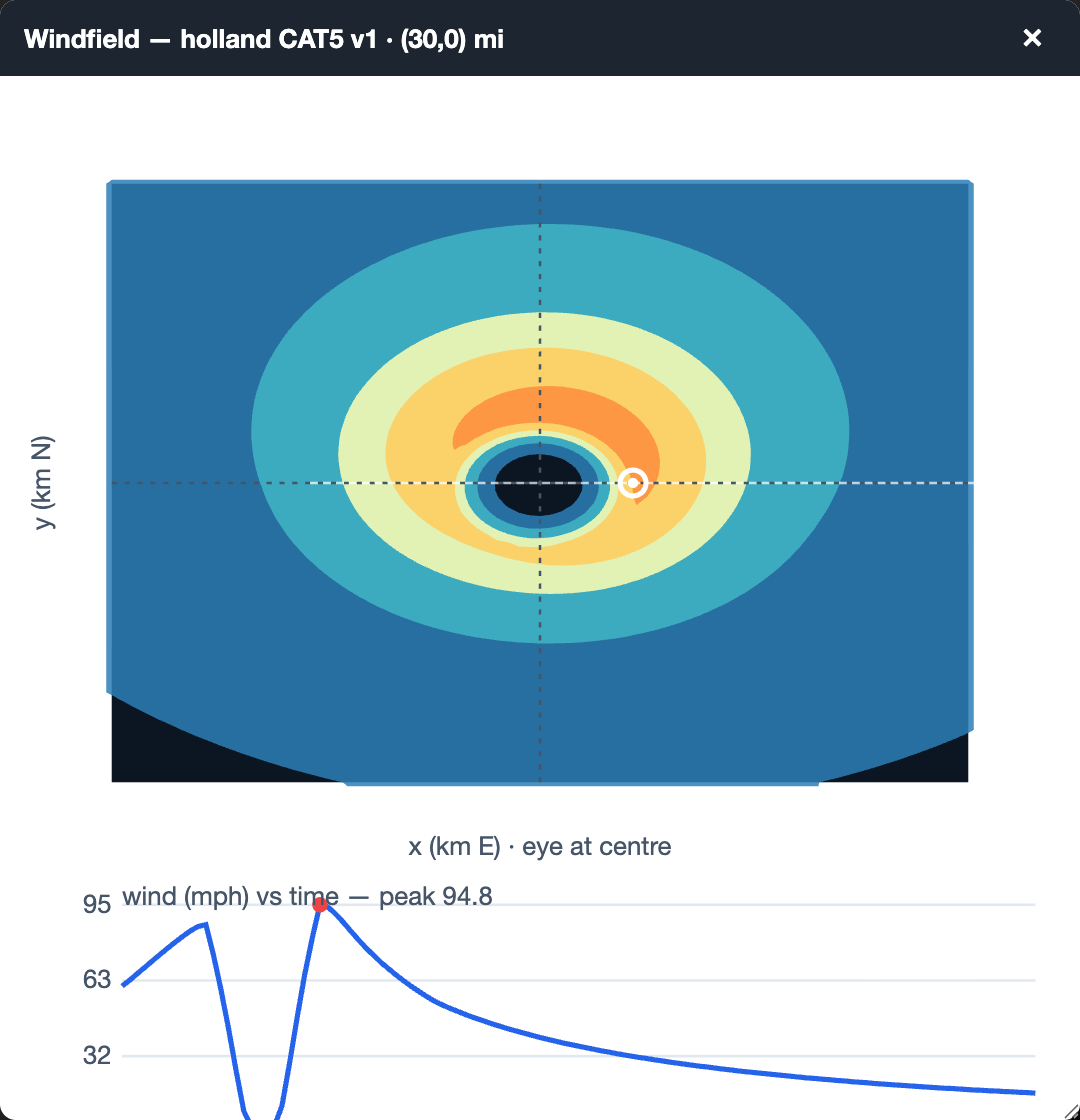
\includegraphics[width=0.46\textwidth]{windfield_popup.png}
\caption{Left: light theme, Powell Category~3 peak-wind points. Right: the
left-click windfield popup---storm-relative isotachs with the clicked vertex
marked at its peak time, plus the per-vertex wind time series.}
\label{fig:light}
\end{figure}
\label{fig:popup}

All data artifacts are reproducible via \texttt{pipeline/build\_all.sh}
(grid, place names, NLCD fetch, roughness, inputs, and the Powell
marine/K\&D/field precomputes), with \texttt{build\_vulnerability.py} for the
loss curve and \texttt{windfield\_ua.py} for the faithful Powell EPR. The app is
served with \texttt{./start} at \url{http://localhost:8012/web/index.html}.
Figures here are captured by \texttt{docs/capture\_figures.py} (Selenium driving
headless Chrome against the running viewer).

\begin{thebibliography}{9}
\bibitem{fchlpm} Florida Commission on Hurricane Loss Projection Methodology (2025).
\emph{Report of Activities}. Standard S-3 and Form S-6.

\bibitem{iman} Iman, R.~L., Johnson, M.~E., and Schroeder, T.~A. (2001).
\emph{Professional Team Demonstration Uncertainty/Sensitivity Analysis}.
\url{https://fchlpm.sbafla.com/media/tepang2l/ua-sa-demo.pdf}

\bibitem{holland} Holland, G.~J. (1980). An analytic model of the wind and pressure
profiles in hurricanes. \emph{Monthly Weather Review}, 108, 1212--1218.

\bibitem{willoughby} Willoughby, H.~E., Darling, R.~W.~R., and Rahn, M.~E. (2006).
Parametric representation of the primary hurricane vortex. Part~II: A new family of
sectionally continuous profiles. \emph{Monthly Weather Review}, 134, 1102--1120.

\bibitem{powell} Powell, M.~D., Houston, S.~H., and Reinhold, T.~A. (1996).
Hurricane Andrew's landfall in South Florida. Part~I: Standardizing the surface
wind observations. \emph{Weather and Forecasting}, 11, 304--328.

\bibitem{vickery} Vickery, P.~J., Wadhera, D., Powell, M.~D., and Chen, Y. (2009).
A hurricane boundary layer and wind field model for use in engineering applications.
\emph{Journal of Applied Meteorology and Climatology}, 48, 381--405.

\bibitem{kaplan} Kaplan, J., and DeMaria, M. (1995). A simple empirical model for
predicting the decay of tropical cyclone winds after landfall.
\emph{Journal of Applied Meteorology}, 34, 2499--2512.

\bibitem{esdu} ESDU (1985). \emph{Characteristics of atmospheric turbulence near the
ground. Part~II: Single point data for strong winds (neutral atmosphere)}. ESDU 85020.

\bibitem{nlcd} Multi-Resolution Land Characteristics Consortium (2023).
\emph{NLCD 2021 Land Cover (CONUS)}. \url{https://www.mrlc.gov}.

\bibitem{aersurface} U.S. Environmental Protection Agency.
\emph{AERSURFACE User's Guide}, land-cover to surface-roughness ($z_0$) tables.
\end{thebibliography}

\end{document}
